\section{Method}

The \textit{Practicum} is divided into three sub areas. The first covers the dissection of the model, extrapolating the summary that would be used to robustly identify the internal structure of the model. The second component was to generate a unique signature for the model that is verified with minor and major changes to both the weights and biases, but also to quickly identify the model structure. The third part was discovering the best method to store they model summaries, so that they can be reused, pulled back and compared with the model currently in development, training or deployment.

The final method investigated in the \textit{Practicum} was application. On top of the original aim of determining the evolutionary tree of the model, other applications such as identifying difference between models that are in the process of being trained, as well as identifying portions of the training or deployment that would assist other methods of observability for model development, trust determination and internal visualisation.

\subsection{Developing a Robust Model Synopsis}
The first part of the delivery required that a model, in this case a CNN model in Keras, can be reduced to an information block that each layer contains a summary of the layer that can record any changes in the weights and biases. The structure of a model consists of a number of standard information points that are consistent across all deep learning processes. While we initially focused on CNNs, it became clear that any model could be used. As shown in the architecture diagram (figure \ref{fig:vgg16Architecture}) showing the popular VGG16 Network\cite{simonyanDeepConvolutionalNetworks2014}, all networks consists of multiple hidden layers representing the black-box of artificial intelligence.

\begin{figure}[!ht]
    \centering
    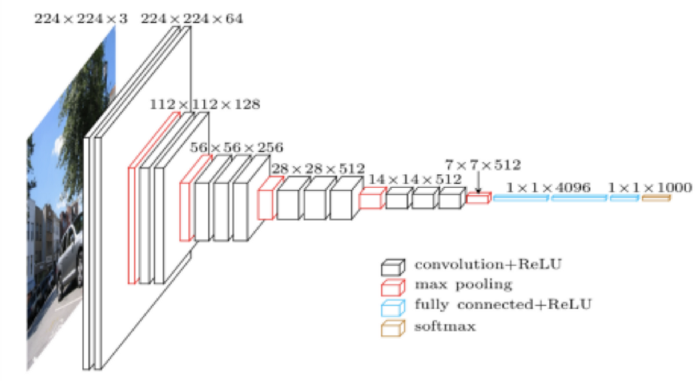
\includegraphics[width=2.5in]{VGG Architecture Overview.png}
    \caption{VGG16 Network Architecture}
    \label{fig:vgg16Architecture}
\end{figure}

The structure of the neural network, while complex, is nearly always of the same format across all recent improvements; not only for convolutional neural networks, but for any type of machine learning application using a modern framework. Even with recurring and shrinking/expanding models, the formula is relatively consistent, as identified below:

\begin{enumerate}
\item An Input Shape. In the case of vision applications, this consists of an image with width, height and colour depth, which is usually three.
\item Dense Application Layers, such as Pooling, Convolution or reduction layers which can contain a heavily connected series of filters, activation functions and weight and bias metrics.
\item Output layers. One or a number of prediction or output layers. In transfer learning, the output layers can change based on the prediction expanding or contracting.
\end{enumerate}

To be able to break down the model, it is necessary to examine the layers for patterns that could be unique or representative. Within each of the layers, there are is a series of sublayers that in the majority of cases are a series of tuples that have a single or multi-dimensional weights, plus optional biases. Theoretically, these values can contain any number, while on inspection, the majority are bound number series that can be tuned up or down in very small increments. It is within these layers that we will extract the layer identification information. For visualisation, the filters do not show information by themselves. For instance the following figure \ref{fig:vggWeightVisualisation}, shows the first layer of a VGG16 network\cite{brownleeHowVisualizeFilters2019}, containing \textit{3x3x3x64} (or 1734) weights.

\begin{figure}[!ht]
    \centering
    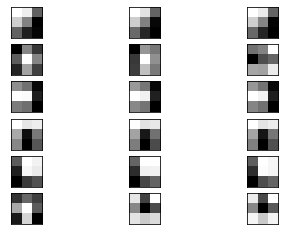
\includegraphics[width=2.5in]{model_values.png}
    \caption{VGG16 First Layer Weights Visualisation}
    \label{fig:vggWeightVisualisation}
\end{figure}

This highlights the importance of not breaking down the layer to each individual layer dimension, as the complexity of the layer gets more complex as the numbers become larger. In the case of our abstraction, we will break down the layer for all values across all dimensions; one for weights, one for bias. To achieve this, we examined a number of mathematical options to identify the data underneath. It was important at this stage to focus on the minimal amount of information that would enable a unique signature to be generated.

Experiments were completed to give an indication of distribution of data, which would assist in visualising the direction of training, in the form of layer-wide histograms or each dimension, and producing a \textit{histogram of gradients}-style overview. These were reduced in favour of two elements - Standard Deviation and Skew. The Standard Deviation formula used was shown below. In both cases experiments were concluded to establish if training a complete end to end network had an effect on the output values that would require a lower granularity of aggregations. 

\begin{equation}
    \label{eqn:stdev}
    \frac1N\sum_{i=1}^n\left(x^i-\overline x\right)^2
\end{equation}

This formula provided a robust mixture that gave of deviation of the smallest change in a 64 bit float, the most commonly used weight and bias internal type used, while still retaining a characteristic was the standards deviation. It also highlighted that if a set of convolutional filter moved all looped in any direction, the standard deviation would remain identical. When filters are used for feature extraction, there is a small potential that a model could be retrained and retain the same standard deviation across all layers.

To counter this we introduced a measure of \textit{skewness} (formula below) to the layer to be recorded. The Pearson's coefficient measure established the relationship between the mode and the standard deviation and gives an indication of the direction \textit{every} combined filter in a layer is veering. As before, unless the feature is two dimensional array, this is not an indication of how the filter performs against an visual input, but instead a protection of the movement of variables from one direction to another.  

\begin{equation}
    \label{eqn:skew}
    G_1=\frac{k_3}{k_2^{3/2}}=\frac{\sqrt{N(N-1)}}{N-2}\frac{m_3}{m_2^{3/2}}.
\end{equation}


Of all the averaging functions available, the implementation of Standard Deviation in the python numpy library was able to reduce every single element to a single 64bit float. A second indication for skew was used to identify the drift of the standard deviation direction, or lack of symmetry,  and is included to ensure that movement of elements that retain the same Standard Deviation will not break the solution.

Trial and Error showed that this was sufficient in training exercises to provide more information. An alternative approach was to develop a histogram of normalised values. The normalisation of the values again would reduce the level of change being recorded in circumstances where the correction of the weights during the learning process is distributed across early feature maps. Binning of distributions, either per dimension can potentially be investigate further, but for this project, the \textit{StdDev} and \textit{Skew} provide enough resolution to work.

To show the difference between this approach, and that shown in other examples for visualisation in the background references, we take a number of early layer in commonly used machine learning models and compare the visualisation with the layer outcomes. For the initial models that were examined, we could tell that the filters behaved very differently between the first convolution of both ResNet50 and VGG16, as shown in figures \ref{fig:vgg16_dcu_image} and \ref{fig:resnet50_dcu_image}.

\begin{figure}[!ht]
    \centering
    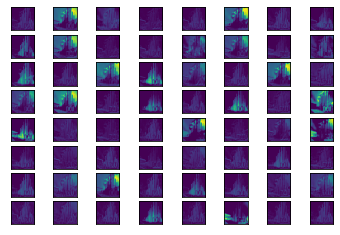
\includegraphics[width=2.5in]{vgg16_dcu_first_layer.png}
    \caption{VGG16 First Layer Image Visualisation}
    \label{fig:vgg16_dcu_image}
\end{figure}

\begin{figure}[!ht]
    \centering
    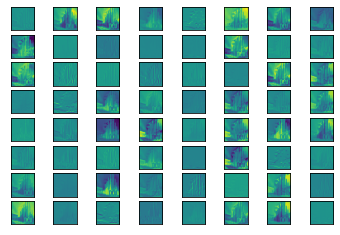
\includegraphics[width=2.5in]{resnet_dcu_first_layer.png}
    \caption{ResNet50 First Layer Image Visualisation}
    \label{fig:resnet50_dcu_image}
\end{figure}

Both first convolutions, loaded with different default imagenet weights give the impression that we can see a visual similarity between feature layers. This is not the case, as even with few parameters, it is not viable to identify when a feature map changes from the weight values or the output image, which when distributed through the neural network, will have a significant effect on the final prediction.

For both of the above images, we can compare the individual Standard Deviation and Skew across each filter, in this case \textit{VGG16 = 0.2067\%, ResNet50 = 0.1111\%} for the Standard Deviation of weights, and \textit{VGG16: -0.0145,ResNet50: -0.1124}. When shown in figure ~\ref{fig:firstlayermodelcomparison}, there is a significant difference in both first layers.

\begin{figure}[!ht]
    \centering
    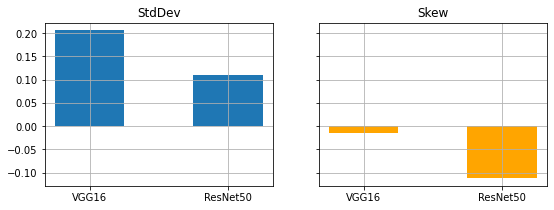
\includegraphics[width=2.5in]{std and skew of first layers.png}
    \caption{Comparison of StdDev and Skew of VGG16, ResNet50}
    \label{fig:firstlayermodelcomparison}
\end{figure}

Once we established that the layers could be represented in this manner, a structure containing both elements for each layer was created. The data structure, including layers with no weights or biases like pooling, padding or normalisation is then used as the one component of generating a signature.

\subsection{Generating a Unique signature}
Once we had all layers reduced to a number of identification values, we aggregated these together and together with a breakdown of the structure, a signature was generated. During this investigation, it was recorded that the process\ref{fig_sig_generator} for extracting an \textit{impression} of the neural network model needs to be one way. If we are focusing on the trust of the system that the model is dependent on, it is necessary to ensure that the model cannot be recreated without the complete data source and process needed to accurately regenerate the model.

The outcome of this project will be establishing if the model is either identical, or the weights and bias are similar. In almost every case, this \textit{\textbf{will not}} be reproducible, instead creating a brand new instance that that path of provenance will be based on.s

\begin{figure}[!ht]
    \centering
    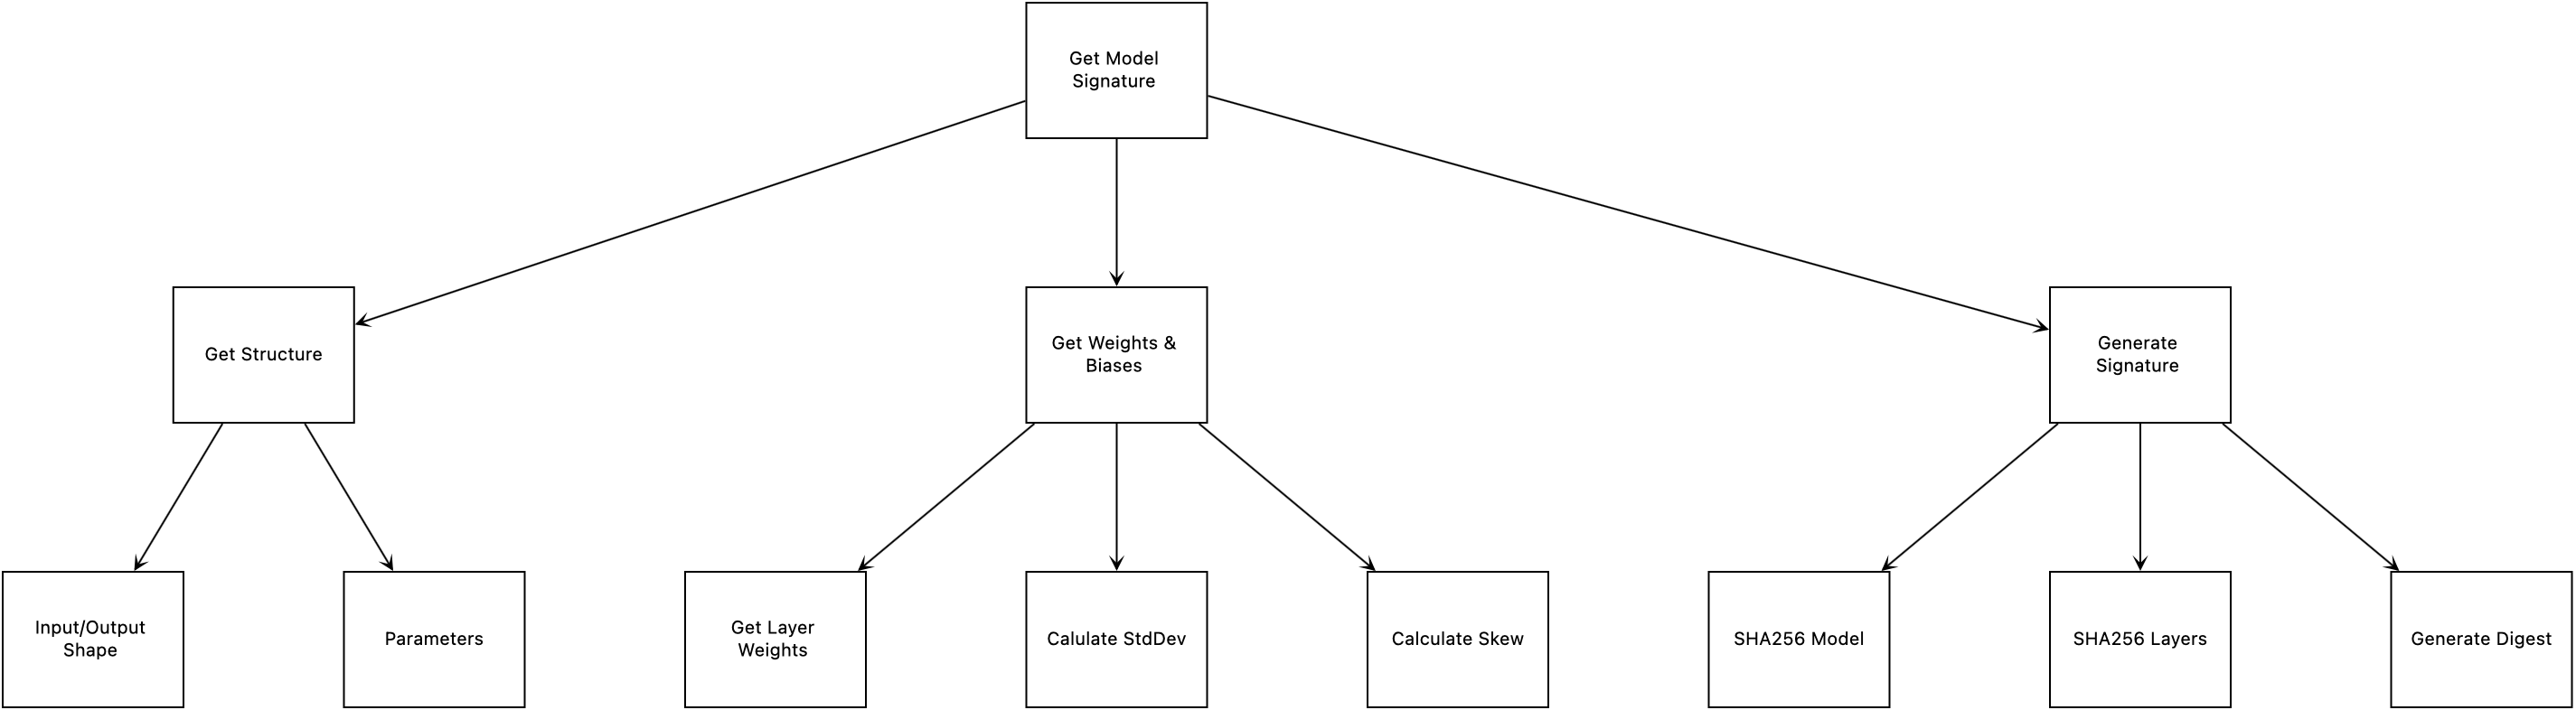
\includegraphics[width=2.5in]{flowchart-3.png}
    \caption{Process for developing Unique Signature}
    \label{fig_sig_generator}
\end{figure}

The flow of generating a new signature is highly dependant on the main hashing algorithm used prior to returning a unique signature. To achieve this, we examined the outcome of running a basic hashing algorithm on each layer, running a SHA-2\cite{technologySecureHashStandard2015} algorithm on the whole stack, and obtaining the basic information synopsis from each layer into an array, and running an SHA-256 algorithm on both the data and the structure array. This method provide the optimal mix between efficiency and utility. While running a number of sha265 update functions will impact on time, particularly in models with a high number of layers to run functions on, it allows minor changes to the layer that don't affect the functionality such as changes names, and other synopsis data. While uniqueness is paramount for the model, unless it is caused by initialisers, then it should be left to one side.

\begin{table}[!ht]
    \centering
    \caption{Data Values stored per Layer}
    \setlength\tabcolsep{0pt} % make LaTeX figure out intercolumn spacing
    \begin{tabular}{@{} p{2cm} p{6.5cm}  @{}}
        \hline
        Metric & Description \\
        \hline
        Weight StdDev  & An indication of the deviation of values, to assist in seeing how the values are weighted \\
        Weight Mean    & The average value of all layers across all dimension \\
        Bias StdDev  & An indication of the deviation of values, to assist in seeing how the values are weighted \\
        Bias Mean    & The average value of all layers across all dimension \\
        Skew   & The skew of the dataset across the entire layer \\
        \hline
    \end{tabular}
\end{table}

The name of the layer was removed as an indicator as the name potentially changes on each pull from the Keras repository. Another aspect to bear in mind that models created without pre-loaded weights will always have a diverse weighting due to the nature of the various initialisers (\textit{Glorut, Uniform etc.}). Initial examination of models created showed a different signature on each restarted system, but a similar signature when a model is created repeatedly. This indicates that the default initialisers remain during repeated creation of models, and using this method would either need to indicate the randomly initialised model is \textit{parentless}, or create a blank slate parent with zero initialiser to compare all similar models.

\subsection{Robustly Recording Changes}
As we now have a method of identifying the model in a broken down format, the next stage is to link the structure to the data model. There are a number of methods of ensuring that the model is recorded. The key part is to take the series of hashes on each layer, combined with the model shape, and generate a signature. The signature is what will be recorded as an immutable value that can be regenerated every time the \textbf{exact} same model is used. With this identification, we can create a list showing the parent and child of the model.

\begin{table}[!ht]
    \centering
    \caption{Structural Data Stored per Layer}
    \setlength\tabcolsep{0pt} % make LaTeX figure out intercolumn spacing
    \begin{tabular}{@{} p{2cm} p{6.5cm}  @{}}
        \hline
        Name & Desc \\
        \hline
        "class" & Class Type of the Layer. There are a number of potential outcomes for the layer type. We do not use the layer type for assessment of the data, purely to identify if the structure has changed. \\
        "input\_shape" & The Shape of the input Array, expressed as a set, i.e. \textit{(None, 224, 224, 3)} for an image input. \\
        "output\_shape" &  The shape of the output layer of the model. This contains either a probability output contain the number of possible outcomes, but can also contain full image data in segmentation and GAN applications. \\
        "trainable" &  A value which indicates if the layer is trainable. Including this boolean change will indicate if transfer learning is being used. \\
        "params" &  The number of parameters in the layer in terms of weights and biases \\
        \hline
    \end{tabular}
\end{table}

To ensure this is done correctly, we have two applications - local, or development and global, or distribution. For global changes single global repository was created in the cloud, where all participants with access can determine if the model being created or downloaded has an existing history. This history can then be used to create a new path of provenance. First, though, the model has to be trained. 

\subsection{Local Changes vs Global Changes}

An additional benefit of the summarisation is to be able to view the model as it is being trained. This is where we introduced a local data repository that can be shared across development teams and organisations to keep track internal models prior to release. This is in comparison with the global model repository, which should only be used for publishing models that require traceability, and not for regular changes.

In keeping with Git vocabulary, local changes are updated with the \verb|push_model(model, [parent])| command, which takes a model and returns a signature and commits the information to a local repository. The local repository stores the abstracted model information set that can be used for local comparisons.
To commit the model to the public repository, either the the \verb|push_model(model, [baseline])| command is used with the \verb|local=False| parameter, or if the model has already be updated elsewhere and the model itself is not available, the \verb|push_to_cloud(signature)| function will commit this with the previously set baseline used as the parent. When applied to the global repository, this will return an error if the parent does not exist, unless permission is granted to create a new ancestor.

Each of the functions are provided as part of a package, encapsulating the data method used. To provide reference storage for the model repositories, we designed multiple MongoDB instances with the same collection structure containing two collections - the signatures and the model data. This enables verification of the evolution path and when necessary pull the model synopsis for comparison.

The signature dataset contains the unique signature, as well as the internal id providing a timestamp. 

\begin{lstlisting}
{"_id":{"$oid":"611063067dbea4ce80c747a0"},
    "signature":"ede69..32 bytes..f0f",
    "parent":null,"username":"brendan.bonner2@mail.dcu.ie",
    "organisation":"Dublin City University",
    "model_source":"Keras Original ResNet50",
    "model_data":{"$oid":"611063067dbea4ce80c7479f"}
}
\end{lstlisting}

The final parament points to the model collection, where a signature is required to find the model. Once a signature is available, it is possible to recover the impression of the complete tree, including the structure and data.

\subsection{Comparing Models}
To ensure there is traceability in between the models, if a parent model is defined, a \textit{b-score} is generated with a degree of difference between the models. The score is based on two factors, the difference between the model structure, and the difference between the two primary parameters for each layer: \textit{StdDev} \& \textit{Skew}. 

\begin{figure}[!ht]
    \centering
    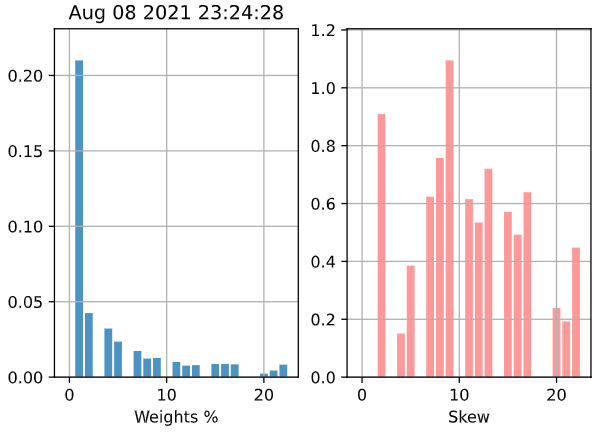
\includegraphics[width=2.5in]{model_changes.png}
    \caption{Difference between model weights and skew per layer}
    \label{fig:weightdiff}
\end{figure}


\subsection{Packaging}

The final area needed was determining how to distribute the mechanism for generating and recording model representation artifacts. The solution was bundled together in a single package called \textit{lifecycle} that allows an existing solution to easily integrate the functions into the standard process. To demonstrate this, we bundled the lifecycle package into a single distributable wheel that was uploaded on a third party python notebook.

As we were not able to guarantee that a local database was available, we were able to setup a cloud instance of MongoDB on their Atlas platform that allowed us to run both local and central repositories in the cloud. This was achieved by adding the following text to the start of the notebook/script:

\begin{lstlisting}
from lifecycle import lifecycle_model
from lifecycle import lifecycle_db

mylifecycle = lifecycle_model()
mydb = lifecycle_db (
    username = '[db username]',
    password = '[password]',
    user='brendan.bonner2@mail.dcu.ie',
    organisation='Dublin City University',
    lifecycle=mylifecycle)

mydb.init_model_db()
\end{lstlisting}

As an example, we were able to apply the package directly to the current leader in the Kaggle Dogs vs Cats challenge\cite{golleMachineLearningAttacks2008}. We were able to add the code example above to the python notebook, add the lifecycle.callback to the fit function. From there we successfully recorded the model prior to training (which was recognised as a ResNet50 network from the global repository), and the training was recorded in the local repository, with two models being recorded as children of the core ResNet50 network on the global repository.

\begin{lstlisting}
from lifecycle.callback import LifecycleCallback

callbacks = [
    LifecycleCallback( mydb)
]
\end{lstlisting}

The result of the initial local stored training, when reduced to 5 epoch, is shown below, with significant training indicated on the model from the base model.In the development of model data sets, we examined every publicly available sample that included training data from the Keras GitHub library, and we were able to show that the lifecycle functions can be applied to CNNs, as well and RNN, Transformers Segmentation classification applications without modifications. Every publicly available preloaded model was also profiled, with results shown in the conclusions.

\begin{lstlisting}
23:24:31 (user:BB)  Weight 0.3657% Skew -0.206
23:24:28 (user:BB), Weight 0.3496% Skew -0.161
23:24:25 (user:BB), Weight 0.3342% Skew -0.131
23:24:21 (user:BB), Weight 0.3194% Skew -0.109
23:24:16 (user:BB), Weight 0.5589% Skew -0.259
23:04:38 (user:Keras), Weight 0.0000% Skew 0.000
\end{lstlisting}
